\subsection{Class number free criterion}

\begin{frame}
\frametitle{Mihăilescu's class number free criterion}

One of Mihăilescu's first steps towards solving the conjecture was eliminating the dependence on the class number in Inkeri's result:
\begin{theorem}[Mihăilescu, 2000]
Let \(\left(x, y, p, q\right)\) be a solution to Catalan's equation with \(p\) and \(q\) distinct odd primes. Then
\[
    p^{q - 1} \equiv 1 \mod{q^2} \text{ and } q^{p - 1} \equiv 1 \mod{p^2}
\]
\end{theorem}
\end{frame}

\begin{frame}
\frametitle{Mihăilescu's class number free criterion}

Mihăilescu's proof \cite{Mihailescu2003_ClassNumberFreeCriterion} relied on a result from the theory of cyclotomic fields which dates back to 1890, Stickelberger's Theorem.
\end{frame}

\begin{frame}
\frametitle{Cyclotomic fields}

Let \(\zeta_p \in \complex\) denote a primitive \(p\)th root of unity. For example, we can take \(\zeta_p \coloneq e^{\frac{2 \pi i}{k}}\)

\begin{definition}
The \(p\)th cyclotomic field is the field extension \(\rationals\left(\zeta_p\right)\)
\end{definition}

\begin{remark}
The minimal polynomial of \(\zeta_p\) is
\[
    f(X) = \frac{X^p - 1}{X - 1} = X^{p - 1} + \dots + X + 1
\]
which is also known as the \emph{cyclotomic polynomial}. This shows that \(\left[\, \rationals\left(\zeta_p\right) : \rationals \,\right] = p - 1\).
\end{remark}
\end{frame}

\begin{frame}[fragile]
\frametitle{Cyclotomic fields}

\begin{figure}
    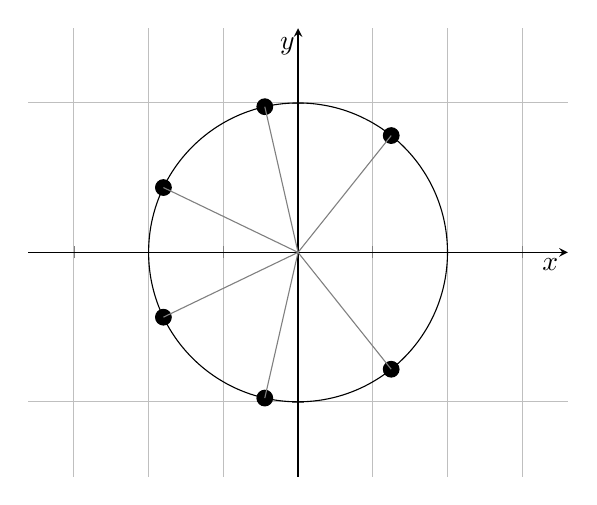
\begin{tikzpicture}
        \begin{axis}[
            grid=both, axis equal,
            ymin=-1.5, ymax=1.5,
            xmin=-1.5, xmax=1.5,
            xticklabel=\empty,yticklabel=\empty,
            axis lines = middle,
            xlabel=\(x\), ylabel=\(y\),
            label style = {at={(ticklabel cs:1,1)}}
        ]  
            \draw (axis cs:0,0) circle [black, radius=1];
            
            \pgfplotsinvokeforeach{1,2,...,6}{
                % Draw the roots of unity
                % Use \pgfplotsforeach as described in https://tex.stackexchange.com/a/170670/263993
                \node[draw, circle, inner sep=2pt, fill] at (axis cs:{cos(deg(2 * pi * #1 / 7))},{sin(deg(2 * pi * #1 /7))}) {};
                
                \draw [thin, gray] (axis cs:0,0) -- (axis cs:{cos(deg(2 * pi * #1 / 7))},{sin(deg(2 * pi * #1 /7))});
            }
        \end{axis}
    \end{tikzpicture}
    \caption*{Primitive roots of unity for \(p = 7\)}
\end{figure}
\end{frame}

\begin{frame}
\frametitle{Cyclotomic fields}

Let \(G\) denote the group
\[
    G = \Gal{\rationals\left(\zeta_p\right)}{\rationals}
\]
i.e.\ the group of field automorphisms of \(\rationals\left(\zeta_p\right)\) which act as the identity on the base field \(\rationals\).

\vspace{1em}

\begin{proposition}
\(G\) is isomorphic to \(\left(\integers/p\integers\right)^{\times}\). Each element \(\sigma_c\) is of the form \(\zeta_p \mapsto \left(\zeta_p\right)^c\) for some \(c \in \Set{1, \dots, p - 1}\).
\end{proposition}
\end{frame}

\begin{frame}
\frametitle{Mihăilescu's class number free criterion}

\begin{definition}
Let \(\integers[G]\) denote the \emph{group ring} of \(G\), i.e.\ the free \(\integers\)-module consisting of finite formal sums of the kind
\[
    \integers[G] = \Set{ \sum_{i = 1}^{k} n_i \sigma_i | n_i \in \integers, \sigma_i \in G}
\]
equipped with the multiplication induced by the group composition.
% TODO: improve explanation
\end{definition}

\vspace{1em}

We can similarly define \(\rationals[G]\), the group ring with coefficients in \(\rationals\).
\end{frame}

\begin{frame}
\frametitle{Mihăilescu's class number free criterion}

Since \(G\) acts on the field \(\rationals\left(\zeta_p\right)\), the group ring \(\integers[G]\) acts on everything defined in terms of it. \\[1em]

\(\integers[G]\) acts naturally on the group of units \(\rationals\left(\zeta_p\right)^{\times}\), the group of units of the ring of integers \(\integers\left[\zeta_p\right]^{\times}\), the group of fractional ideals, the class group etc. \\[1em]

For example, for a unit \(\alpha \in \integers\left[\zeta_p\right]^{\times}\), we have
\[
    \alpha^{\sum_{i = 1}^{k} n_i \sigma_i} = \sigma_1 (\alpha)^{n_1} \cdot \hdots \cdot \sigma_k (\alpha)^{n_k}
\]
\end{frame}

\begin{frame}
\frametitle{Stickelberger element}

\begin{definition}
The Stickelberger element is
\[
    \theta = \sum_{c = 1}^{p - 1} \left\{\frac{c}{p}\right\} \cdot \sigma_{c}^{-1} \in \rationals[G]
\]
\end{definition}
\begin{definition}
The Stickelberger ideal is
\[
    I_{S} = \integers[G] \cap \theta \, \integers[G]
\]
\end{definition}
\end{frame}

\begin{frame}
\frametitle{Stickelberger's Theorem}

\begin{theorem}[Stickelberger, 1890]
The Stickelberger ideal annihilates the class group of \(\rationals\left(\zeta_p\right)\).
\end{theorem}

\vspace{1em}

In other words, for every fractional ideal \(M\), there exists a \(\Theta \in I_S\) such that \(M^{I_S}\) is principal.
\end{frame}

\begin{frame}
\frametitle{Stickelberger's Theorem}

Stickelberger proved his theorem by looking at Gauss sums, i.e.\ sums of the form
\[
    G(\chi) = -\sum_{a \in \finitefield{p}} \chi(a) \cdot \zeta_p^{a}
\]
for \(\chi \in \finitefield{p} \to \complex^{\times}\) a character. See \cite{Washington1997} for a detailed proof.
\end{frame}

\begin{frame}
\frametitle{Mihăilescu's class number free criterion}

We have the decomposition
\[
    \frac{x^p - 1}{p (x - 1)} = \prod_{i = 1}^{p - 1} \frac{x - \zeta_p^i}{1 - \zeta_p^i}
\]
and by Cassel's relations
\[
    \frac{x^p - 1}{p (x - 1)} = u^q
\]
for some \(u \in \integers\). Hence,
\[
    \prod_{i = 1}^{p - 1} \frac{x - \zeta_p^i}{1 - \zeta_p^i} = u^q
\]
\end{frame}

\begin{frame}
\frametitle{Mihăilescu's class number free criterion}

The ideals
\[
    \beta_i = \left(\frac{x - \zeta_p^i}{1 - \zeta_p^i}\right) \integers\left[\zeta_p\right]
\]
are coprime. By the unique factorisation of ideals, they must all be \(q\) powers:
\[
    \beta_i = \symfrak{u}_i^q
\]
Mihăilescu proceeds by applying elements \(\Theta\) from the Stickelberger ideal to these ideals and performing a few calculations in the spirit of Hyyrö and Inkeri's proofs.
\end{frame}
